\documentclass[11pt]{article}

% load some asm stuff -
\usepackage{amssymb}
\usepackage{amsmath}
\usepackage{amsthm}
%\usepackage{palatino,lettrine}
\usepackage{fancyhdr}
\usepackage{epsfig}
\usepackage[square,sort,comma,numbers]{natbib}
\usepackage{simplemargins}
\usepackage{setspace}
\usepackage{wrapfig}
\usepackage{hyperref}
%\usepackage{boiboites}
\usepackage[margin=0pt,font=small,labelfont=bf]{caption}
\newcommand{\boldindex}[1]{\textbf{\hyperpage{#1}}}
\usepackage{makeidx}\makeindex
\bibliographystyle{plos2015}


\usepackage{algpseudocode}
\usepackage{algorithm}

% Set the size
%\textwidth = 6.75 in
%\textheight = 9.75 in
%\oddsidemargin = 0.0 in
%\evensidemargin = 0.0 in
%\topmargin = 0.01 in
%\headheight = 0.0 in
%\headsep = 0.25 in
%\parskip = 0.15in
% \doublespace
\setallmargins{1in}

\newtheorem{example}{Example}[section]
\newtheorem{thm}{Theorem}[section]
\newtheorem{property}{Property}[section]

\theoremstyle{definition}
\newtheorem{defn}[thm]{Definition}

\makeatletter
% \renewcommand\subsection{\@startsection
% 	{subsection}{2}{0mm}
% 	{-0.05in}
% 	{0.1\baselineskip}
% 	{\normalfont\normalsize\bfseries}}
\renewcommand\subsubsection{\@startsection
	{subsubsection}{2}{0mm}
	{-0.05in}
	{-0.5\baselineskip}
	{\normalfont\normalsize\itshape\bfseries}}
\renewcommand\paragraph{\@startsection
	{paragraph}{2}{0mm}
	{-0.05in}
	{-0.5\baselineskip}
	{\normalfont\normalsize\itshape}}
\makeatother
\linespread{1.1}

\fancypagestyle{proposal}{\fancyhf{}%
	\fancyhead[RO,LE]{\thepage}%
	\fancyhead[LO,RE]{CHEME 5660 Financial Decision Approaches}%
	\renewcommand\headrulewidth{1pt}}
\pagestyle{proposal}

\usepackage{mdframed}
\definecolor{lgray}{rgb}{0.92,0.92,0.92}
\definecolor{antiquewhite}{rgb}{0.98,0.92,0.84}
\definecolor{lightskyblue}{rgb}{0.93,0.95,0.99}

% defn environment
\mdfdefinestyle{theoremstyle}{% 
    linecolor=black,linewidth=1pt,% 
    frametitlerule=true,% 
    frametitlebackgroundcolor=lgray, 
    innertopmargin=\topskip,} 
\mdtheorem[style=theoremstyle]{definition}{Definition}

% concept environment
\mdfdefinestyle{conceptstyle}{% 
    linecolor=black,linewidth=1pt,% 
    frametitlerule=true,% 
    frametitlebackgroundcolor=lightskyblue, 
    innertopmargin=\topskip,} 
\mdtheorem[style=conceptstyle]{concept}{Concept}
\newcommand{\newterm}[1]{{\it #1}}

% Single space'd bib -
\setlength\bibsep{0pt}

\renewcommand{\rmdefault}{phv}\renewcommand{\sfdefault}{phv}
%\newboxedtheorem[boxcolor=black, background=gray!5,titlebackground=orange!20,titleboxcolor = black]{color_box_example}{Example}{test}

% Change the number format in the ref list -
\renewcommand{\bibnumfmt}[1]{#1.}

% Change Figure to Fig.
\renewcommand{\figurename}{Fig.}
\usepackage{enumitem}
\setlist{noitemsep} % or \setlist{noitemsep} to leave space around whole list

%Joycelyn Chan, Joshua Lequieu, Michael Paull, Chidanand Balaji, Ryan Tasseff
%Our derivation follows closely the earlier development of Fredrickson \citep{Fredrickson:1976fk}.

% Begin ...
\begin{document}

%\begin{titlepage}
{\par\centering\textbf{\Large Unit 4: Financial Decision Approaches}}
\vspace{0.2in}
{\par \centering \large{Jeffrey D. Varner}}
\vspace{0.05in}
{\par \centering \large{Smith School of Chemical and Biomolecular Engineering}}
{\par \centering \large{Cornell University, Ithaca NY 14853}}
% \vspace{0.1in}
% {\par \centering \small{Copyright \copyright\ Jeffrey Varner 2018. All Rights Reserved.}}\\

%\end{titlepage}
\date{}
\thispagestyle{empty}

\setcounter{page}{1}

\tableofcontents
\clearpage
\listoffigures
\clearpage
\listofalgorithms
\clearpage

\section{Introduction}
Decision making in random systems, particularly in financial contexts, involves navigating environments where outcomes are influenced by both predictable and unpredictable factors. 
Random systems are characterized by their reliance on probability distributions to describe the behavior of various elements. 
In finance, this could involve modeling the price movements of assets, interest rates, or other economic indicators. 
The goal is to understand and predict these movements to make informed decisions.
Techniques such as Monte Carlo simulations, which use random sampling to estimate the probability of different outcomes, which we have already discussed, are commonly employed to assess the impact of uncertainty on investment strategies.
In this unit, we will explore the use of Markov decision processes (MDPs) to model and solve decision-making problems in financial contexts.
MDPs are a powerful tool for modeling sequential decision-making problems where outcomes are influenced by both random and controlled factors.
However, MDPs require a detailed understanding of the underlying system dynamics and the ability to model these dynamics accurately.
Thus, we will also explore model-free approaches, such as reinforcement learning, which learn by interacting with the environment and do not require explicit knowledge of the system dynamics.
Let's start by exploring the fundamental concepts of Markov chains and Markov decision processes
in Section \ref{sec:markov-decision-processes}.
We'll then move on to model-free approaches such as Bandit problems in Section \ref{sec:bandit-problems} 
and reinforcement learning in Section \ref{sec:reinforcement-learning}.

\section{Markov Decision Processes}\label{sec:markov-decision-processes}
Markov chains, Markov models, and Markov decision processes are bedrock concepts in the field of stochastic processes, which are essential for understanding a wide range of applications in mathematics, economics, computer science, and beyond. 
These concepts provide a framework for modeling systems that undergo transitions from one state to another in a probabilistic manner.
Let's start by looking Markov chains, and work our way up to Markov decision processes.

\subsection{Markov Chains and Markov Models}
A Markov chain is a type of stochastic process where the future state of the system depends only on the present state and not on the sequence of events that preceded it. 
This property is known as the Markov property. 
Markov chains are characterized by a set of states and transition probabilities between these states, 
which can be represented using a transition matrix. They are used to model various phenomena such as population dynamics, queueing systems, and random walks (which is the application we are most interested in).


\begin{figure}[h]
    \centering
    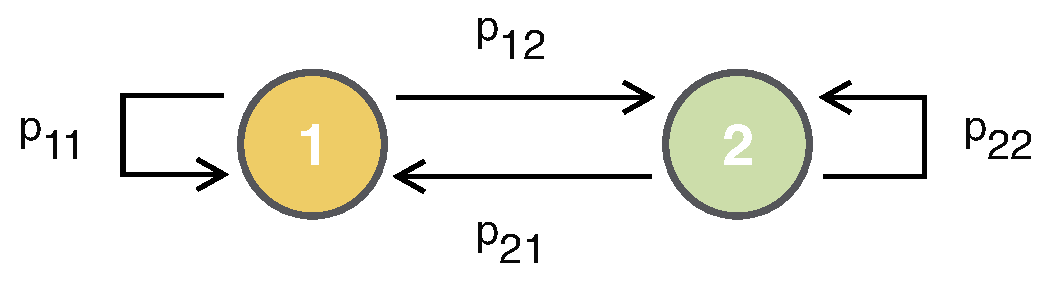
\includegraphics[width=0.75\textwidth]{./figs/Fig-Discrete-MarkovChain-Schematic.pdf}
    \caption{Schematic of a discrete two-state time-invariant Markov model; 
    $p_{ij}$ denotes the time-invariant transition probability between state $i$ and $j$.}\label{fig-discrete-markov-model}
\end{figure}

\subsubsection*{Discrete-Time Markov Chains}
A discrete-time Markov chain is a sequence of random variables $X_{1},\dotsc, X_{n}$ with 
the \href{https://en.wikipedia.org/wiki/Markov_property}{Markov property}, 
i.e., the probability of moving to the next state depends only on the present and not past states:
\begin{equation}
P(X_{n+1} = x | X_{1}=x_{1}, \dots, X_{n}=x_{n}) = P(X_{n+1} = x | X_{n}=y)
\end{equation}
For finite state spaces $\mathcal{S}$, the probability of moving from the state(s) $i\rightarrow{j}$ in the next turn, 
is encoded in the $|\mathcal{S}|\times|\mathcal{S}|$ transition matrix $p_{ij}\in\mathbf{P}$: 
\begin{equation}
p_{ij} = P(X_{n+1}~=~j~|~X_{n}~=~i)
\end{equation}
where $p_{ij}\geq{0}$ for all $i,j\in\mathcal{S}$. The transition matrix $\mathbf{P}$ has interesting properties. First, the rows of transition matrix $\mathbf{P}$ sum to unity, i.e., each row encodes the probability of all possible outcomes in the next turn.
Thus, it must sum to one. Second, if the transition matrix  $\mathbf{P}$ is invariant, $p_{ij}$ doesn't change as $n\rightarrow{n+1}~\forall{n}$.
Finally, for a non-periodic Markov chain with a finite state space $\mathcal{S}$ and an invariant state transition matrix $\mathbf{P}$,
the state vector at time $j$, denoted by $\mathbf{\pi}_{j}$, has the property:
\begin{equation}
\sum_{s\in\mathcal{S}}\pi_{sj} = 1\qquad\forall{j}
\end{equation}
where $\pi_{sj}\geq{0},\forall{s}\in\mathcal{S}$. The state of the Markov chain at time step $n+1$, denoted by $\mathbf{\pi}_{n+1}$, is given by:
\begin{equation}
\mathbf{\pi}_{n+1} = \mathbf{\pi}_{1}\cdot\left(\mathbf{P}\right)^n
\end{equation}
where $\mathbf{\pi}_{1}$ is the initial state vector, and $\left(\mathbf{P}\right)^n$ is the transition matrix raised to the $n$-th power.
Finally, for a non-periodic chain, a unique stationary distribution $\bar{\pi}$ exists; in the limit of large $k$ the $\mathbf{P}^{k}$ 
converges to a rank-one matrix in which each row is the stationary distribution $\bar{\pi}$:
\begin{equation}
\lim_{k\rightarrow\infty} \mathbf{P}^{k} = \mathbf{1}\otimes{\bar{\pi}}
\end{equation} 
where $\mathbf{1}$ is a column vector of all 1s and $\otimes$ denotes the outer product.

\subsubsection*{Hidden Markov Models.}
Markov models extend the concept of Markov chains by incorporating additional complexities such as potentially continuous state spaces, time parameters or observable versus hidden states. 
These models are widely used in fields like economics and finance to predict future states of a system based on current observations. 
They can also be employed in machine learning for tasks like sequence prediction and natural language processing. 

One common example of a Markov model (which we will use) is the hidden Markov model (HMM).
A Hidden Markov Model (HMM) is a statistical model used to represent systems where the underlying processes are not directly observable, but can be inferred through observable sequences. 
The model is based on the concept of a latent Markov process, where the hidden states influence the observable outputs. 
In HMMs, the relationship between the hidden states and observations is defined through two sets of probabilities: 
transition probabilities, which describe the likelihood of moving from one hidden state to another, and emission probabilities, 
which describe the likelihood of an observation given a hidden state (see Definition \ref{defn-hidden-markov-model}). 

\begin{definition}[Hidden Markov Model]\label{defn-hidden-markov-model}
A hidden Markov model is defined by the tuple: $\mathcal{M} = (\mathcal{S},\mathcal{O},\mathbf{P},\mathbf{E})$. 
\begin{itemize}
\item{The state space $\mathcal{S}$ is the set of all possible \textit{hidden} states $s$ that the model $\mathcal{M}$ contains}
\item{The observation space $\mathcal{O}$ is the set of all possible \textit{observable} states $o$ that the model $\mathcal{M}$ can emit}
\item{The transition matrix $\mathbf{P}$ encodes the probability of moving from one hidden state to another hidden state at the next time step where $p_{ij} = P(X_{n+1} = j | X_{n} = i)$ must satisfy:
\begin{equation}
\sum_{j\in\mathcal{S}} p_{ij} = 1\qquad\forall{i\in\mathcal{S}}
\end{equation}}
\item{The emission matrix $\mathbf{E}$ encodes the probability of emitting an observable state
$o\in\mathcal{O}$ from a hidden state $s\in\mathcal{S}$ where the elements $e_{ij} = P(Y = j\,| X = i)$ must satisfy:
\begin{equation}
\sum_{j\in\mathcal{O}} e_{ij} = 1\qquad\forall{i\in\mathcal{S}}
\end{equation}}
\end{itemize}   
\end{definition}
 
Let's consider the following pseudocode implementation for a hidden Markov model simulation (Algorithm \ref{algo-hidden-markov-model}).
\begin{algorithm}[H]
    \caption{Hidden Markov Model}\label{algo-hidden-markov-model}
    \begin{algorithmic}[1]
        \Procedure{markov-simulation}{$\mathbf{A},\mathbf{E},\bar{\pi}, n$}

            \State{$\dim\mathcal{S},\,\dim\mathcal{O}\gets\texttt{size}(\mathbf{E})$}\Comment{Dimension of the emission matrix $\mathbf{E}$ using $\texttt{size}$}
            \Statex
            \For{$s=1$ to $\dim\mathcal{S}$}
                \State{$d_{H}(s)\gets\texttt{Categorical}(\mathbf{A}[s,\dots])$}\Comment{Construct a categorical distribution $d_{H}$}
                \State{$d_{O}(s)\gets\texttt{Categorical}(\mathbf{E}[s,\dots])$}\Comment{Construct a categorical distribution $d_{O}$}
            \EndFor
            \Statex
            \State{$s\gets\texttt{rand}(\bar{\pi})$}\Comment{Generate initial state $s$ from $\bar{\pi}$ using $\texttt{rand}$ function}
            \For{$i=1$ to $n$}
                \State{$s^{\prime}\gets\texttt{rand}\circ{d_{H}}(s)$}\Comment{Generate next state $s^{\prime}$ by sampling $d_{H}$ distribution}
                \State{$o\gets\texttt{rand}\circ{d_{O}}(s^{\prime})$}\Comment{Generate observation $o$ by sampling $d_{O}$ distribution}
                \State{$s\gets{s^{\prime}}$}\Comment{Update state $s$ to $s^{\prime}$}
            \EndFor
        \EndProcedure
    \end{algorithmic}
\end{algorithm}

The stationary distribution $\bar{\pi}$ is a probability distribution over the state space $\mathcal{S}$, where each state $s\in\mathcal{S}$ occurs with probability $\bar{\pi}_{s}$. The stationary distribution $\bar{\pi}$ describes the steady-state behavior of the Markov chain.
We model the rows of $\mathbf{P}$, $\mathbf{E}$ and the stationary distribution $\bar{\pi}$ using \href{https://en.wikipedia.org/wiki/Categorical_distribution}{Categorical distributions}. 
Categorical distributions are discrete probability distributions modeling the probability of a random variable taking a particular outcome $k\in\mathcal{K}$:
\begin{equation}
P(X = k) = \pi_{k}\qquad\text{where}\qquad\sum_{k\in\mathcal{K}}\pi_{k} = 1
\end{equation}
Sampling from a categorical distribution constructed from the rows of $\mathbf{P}$ (or $\mathbf{E}$)
will return the next state $s^{\prime}$ (or observation $o$).

\subsection{Markov Decision Processes}
A Markov decision process (MDP) provides a mathematical framework for modeling decision-making in situations 
where outcomes are partly random and partly under the control of a decision-maker. 
MDPs take their name from the mathematician \href{https://en.wikipedia.org/wiki/Andrey_Markov}{Andrey Markov}, 
as they are an extension of \href{https://en.wikipedia.org/wiki/Markov_chain}{Markov chains}, 
a stochastic model which describes a sequence of possible events in which the probability of each event depends only on the 
system state in the previous event.

At each time step, let's assume the system in some state $s$ in a set of possible states $s\in\mathcal{S}$ and the decision maker 
may choose any action $a$ from a set of possible actions $a\in\mathcal{A}$ that are available in state $s$. 
The system responds at the next time step by potentially moving into a new state $s^{\prime}$ and rewarding the decision maker $R_{a}\left(s, s^{\prime}\right)$.
The probability that the system moves into a new state $s^{\prime}$ depends upon the chosen action $a$ and the current state $s$; 
this probability is governed by a state transition function $P_{a}\left(s,s^{\prime}\right)$.

\begin{definition}[Markov Decision Process Tuple]
A Markov decision process is the tuple $\left(\mathcal{S}, \mathcal{A}, R_{a}\left(s, s^{\prime}\right), T_{a}\left(s,s^{\prime}\right), \gamma\right)$ where:
\begin{itemize}
\item{The state space $\mathcal{S}$ is the set of all possible states $s$ that a system can exist in}
\item{The action space $\mathcal{A}$ is the set of all possible actions $a$ that are available to the agent, where $\mathcal{A}_{s} \subseteq \mathcal{A}$ is the subset of the action space $\mathcal{A}$ that is accessible from state $s$.}
\item{An expected immediate reward $R_{a}\left(s, s^{\prime}\right)$ is received after transitioning from state $s\rightarrow{s}^{\prime}$ due to action $a$.}
\item{The transition $T_{a}\left(s,s^{\prime}\right) = P(s_{t+1} = s^{\prime}~|~s_{t}=s,a_{t} = a)$ denotes the probability that action $a$ in state $s$ at time $t$ will result in state $s^{\prime}$ at time $t+1$}
\item{The quantity $\gamma$ is a discount factor; the discount factor is used to weight the future expected utility.}
\end{itemize}
Finally, a policy function $\pi$ is the (potentially probabilistic) mapping from states $s\in\mathcal{S}$ to actions $a\in\mathcal{A}$ used by the agent to solve the decision task. 
\end{definition}

\subsection{Policies and Value Functions}
One immediate question that jumps out is what is a policy function $\pi$, and how do we find the best possible policy for our decision problem? 
To do this, we need a way to estimate how good (or bad) a particular policy is; the approach we use is called policy evaluation. 
Let's denote the expected utility gained by executing some policy $\pi(s)$ from state $s$ as $U^{\pi}(s)$. 
Then, an optimal policy function $\pi^{\star}$ is one that maximizes the expected utility:
\begin{equation}
\pi^{\star}\left(s\right) = \text{arg max}~U^{\pi}(s)
\end{equation}
for all $s\in\mathcal{S}$. We can iteratively compute the utility of a policy $\pi$. 
If the agent makes a single move, the utility will be the reward the agent receives by implementing policy $\pi$:
\begin{equation}
U_{1}^{\pi}(s) = R(s,\pi(s))
\end{equation}
However, if we let the agent perform two, three, or $k$ possible iterations, we get a lookahead equation which relates the value of 
the utility at iteration $k$ to $k+1$:
\begin{equation}
U_{k+1}^{\pi}(s) = R(s,\pi(s)) + \gamma\sum_{s^{\prime}\in\mathcal{S}}T(s^{\prime} | s, \pi(s))U_{k}^{\pi}(s^{\prime})
\end{equation}
As $k\rightarrow\infty$ the lookahead utility converges to a stationary value $U^{\pi}(s)$ (Definition \ref{def:converged-policy-evaluation}).
\begin{definition}[Converged Policy Evaluation]\label{def:converged-policy-evaluation}
Suppose we have a Markov decision process with the tuple $\left(\mathcal{S}, \mathcal{A}, R_{a}\left(s, s^{\prime}\right), T_{a}\left(s,s^{\prime}\right), \gamma\right)$. 
Then, the utility of the policy function $\pi$ equals:
\begin{equation}
U^{\pi}(s) = R(s,\pi(s)) + \gamma\sum_{s^{\prime}\in\mathcal{S}}T(s^{\prime} | s, \pi(s))U^{\pi}(s^{\prime})
\end{equation}
The utility associated with an optimal policy $\pi^{\star}$ is called the optimal utility $U^{\star}$. 
\end{definition}

Definition \ref{def:converged-policy-evaluation} gives us a method to compute the utility for a particular policy $U^{\pi}(s)$. 
However, suppose we were given the utility and wanted to estimate the policy $\pi(s)$ from that utility. 
Given a utility $U$, we can estimate a policy $\pi(s)$ using the $Q$-function (action-value function):
\begin{equation}\label{eqn-action-value-function}
Q(s,a) = R(s,a) + \gamma\sum_{s^{\prime}\in\mathcal{S}}T(s^{\prime} | s, a)U(s^{\prime})
\end{equation}
For discrete state and action spaces, \eqref{eqn-action-value-function} gives a $|\mathcal{S}|\times|\mathcal{A}|$ array, where the utility is given by:
\begin{equation}\label{eqn-utility-from-Q}
U(s) = \max_{a} Q(s,a)
\end{equation}
and the policy $\pi(s)$ is:
\begin{equation}\label{eqn-policy-from-Q}
\pi(s) = \text{arg}\max_{a}Q(s,a)
\end{equation}

\subsection{Summary}
Fill me in

\section{Bandit Problems}\label{sec:bandit-problems}
The \href{https://en.wikipedia.org/wiki/Multi-armed_bandit}{multi-armed bandit problem} is a fundamental problem in machine learning and decision-making. 
It refers to a scenario where an agent must repeatedly choose between multiple actions, each with an unknown reward distribution. 
Each action can be considered a slot machine, or a one-armed bandit with potentially different payout distributions. 
The goal of the agent is to maximize its total reward over time while learning the reward distributions of the different actions. 
This presents a tradeoff between exploitation, where the agent chooses the action with the highest estimated reward so far, and exploration, 
where it selects an action with an uncertain reward to learn more about its distribution. The multi-armed bandit problem has practical applications in various fields, 
such as clinical trials, online advertising, and recommender systems.

\subsection{Binary Bernoulli Bandits}\label{sec:binary-bernoulli-bandits}
A bandit problem is a sequential game, played between an agent and the world, over $T$ turns called the horizon.
In each turn the agent chooses an action $a\in\mathcal{A}$, implements this action, and receives a reward $r$ from the world.
The goal of the agent is to maximize the total reward over the horizon, i.e., the agent learns the differnce between good and bad actions based on the rewards it receives.
There are many different bandit problem varients, so let's focus on a particular sub-type of bandit problem, namely, 
the Bernoulli bandit problem (Definition \ref{def:bernoulli-bandit-problem}).

\begin{definition}[Bernoulli Bandit Problem]\label{def:bernoulli-bandit-problem}
A binary Bernoulli bandit problem is a multi-arm bandit problem where each action $a\in\mathcal{A}$ has a binary reward distribution
governed by a \href{https://en.wikipedia.org/wiki/Bernoulli_distribution}{Bernoulli random variable} with unknown success parameter $p_{a}$:
\begin{itemize}
\item{An agent chooses between $K$ possible actions $\mathcal{A}=\left\{a_{1},a_{2},\dots,a_{K}\right\}$ where the success or failure of any action $a_{i}\in\mathcal{A}$
is governed by \href{https://en.wikipedia.org/wiki/Bernoulli_distribution}{Bernoulli random variable} with unknown success parameter $p_{a_{i}}$.}
\item{During the game, the agent learns the success probabilities $p_{a_{i}}$ by experimenting with the world. If action $a$ is successful, the agent receives a reward $r=1$, otherwise $r=0$.}
\item{The success probabilities are modeled by the agent as $p_{a}\sim\text{Beta}(\alpha,\beta)$, 
where the agent learns updates to the parameters $(\alpha,\beta)$ of the \href{https://en.wikipedia.org/wiki/Beta_distribution}{$\text{Beta}$ distribution}
by experimenting with the world.}
\end{itemize}
The agent's objective is to choose actions that maximize the cumulative reward over the game \textit{horizon}.
\end{definition}

\subsection{Thompson Sampling}\label{sec:exploration-and-exploitation}
In decision-making, the multi-armed bandit problem serves as a classic framework for understanding the trade-off between exploration and exploitation. 
The challenge for the decision agent lies in balancing the exploration of new actions to gather information and the exploitation of known actions to maximize rewards. 
Thompson Sampling, which was first published in the context of clincal trials in the 1930s \citep{Thompson-1933}, has emerged as a prominent approach to address this dilemma \citep{Russo-Thompson-Sampling}. 
It operates by maintaining probability distributions (implemented as \href{https://en.wikipedia.org/wiki/Beta_distribution}{$\text{Beta}$ distributions} in our case) over the potential success probabilities of each action $p_{a}$ and sequentially updates these distributions based on observed outcomes. 
By sampling from these distributions, Thompson Sampling probabilistically favors options that appear promising, thus efficiently navigating the exploration-exploitation trade-off. 
The algorithm is simple, intuitive, and has been shown to perform well in practice, and it has some theoretical guarantees of optimality under certain conditions \citep{Agrawal-2012}.
A pseudocode implementation of $\epsilon$-Greedy Thompson Sampling is provided in Algorithm \ref{algo:eps-greedy-Thompson-sampling}.
\begin{algorithm}[H]
    \caption{$\epsilon$-Greedy Thompson Sampling}\label{algo:eps-greedy-Thompson-sampling}
    \begin{algorithmic}[1]
        \normalsize
        \Procedure{$\epsilon$-Greedy Thompson Sampling}{}
        \State Initialize the $\alpha, \beta$-vectors, the success $\mathbf{S}$ and fail $\mathbf{F}$ vectors and action set $\mathcal{A}$
        \For{$k \in 1~\text{to}~\text{horizon}$}\Comment{{\color{black} Play the game for $\text{horizon}$ rounds}}
        \State{$a \gets \texttt{nothing}$}
        \If{$\texttt{rand} < \epsilon$}\Comment{{\color{black} With threshold $\epsilon$, we explore}}
            \State{$a \gets \texttt{uniform}(\mathcal{A})$}\Comment{{\color{black} Exploration generates a uniform random $a\in\mathcal{A}$}}
        \Else\Comment{{\color{black} With probability $1-\epsilon$, we exploit}}
            \State{$\mathbf{p}\gets\left\{\text{Beta}(\alpha(k)+\mathbf{S}(k),\beta(k)+\mathbf{F}(k))\right\}_{k=1}^{\dim\mathcal{A}}$}\Comment{{\color{black} Draw $\dim\mathcal{A}$ samples}}
            \State{$a\gets\arg\max_{a}\mathbf{p}$}\Comment{{\color{black} Select the action with the highest success probability}}
        \EndIf
        \State{$r\gets\texttt{world}(a)$}\Comment{{\color{black} Observe the reward $r\in{0,1}$ from the \texttt{world} from action $a$}}
        \State{$\mathbf{S}(a)\gets\mathbf{S}(a)+r$}\Comment{{\color{black} Update the success count for action $a$}}
        \State{$\mathbf{F}(a)\gets\mathbf{F}(a)+(1-r)$}\Comment{{\color{black} Update the fail count for action $a$}}
        \EndFor
        \EndProcedure
    \end{algorithmic}
\end{algorithm}

\subsubsection*{Why a $\text{Beta}$ distribution?}\label{sec:beta-distribution}
Our implementation of Thompson Sampling uses a $\text{Beta}$ distribution to model the success probabilities of each action, i.e., 
$\text{Beta}(\alpha,\beta)$ distributions is are the \texttt{brain} of the agent that learn the best action $a\in\mathcal{A}$ to take over
the horizon of the training run.

\subsection{Summary}
Bandit problems, particularly the multi-armed bandit (MAB) problem, are classic examples of sequential decision-making challenges that involve balancing exploration and exploitation. 
In these problems, a decision-maker must choose between multiple options (or "arms"), each with an unknown probability distribution of rewards, with the goal of maximizing cumulative rewards over time. 
This setup is analogous to a gambler deciding which slot machine to play in a casino to maximize their winnings. 
The challenge lies in determining the best strategy to gather information about the reward distributions while also capitalizing on known information to maximize returns.

\section{Model Free Reinforcement Learning}\label{sec:reinforcement-learning}
\subsection{Q-Learning in Discrete Spaces}\label{sec:q-learning}
\subsection{Q-Learning in Continuous Spaces}\label{sec:q-learning-continuous}
\subsection{Applications of Q-Learning}\label{sec:applications-of-q-learning}
\subsection{Summary}

\clearpage
\bibliography{References_v1}

\end{document}